\chapter{Challenges}\label{sec-challenges}

According to the pipeline of software reverse engineering and existing
literature, several challenges inhibit the further improvement of the accuracy
and reliability of reverse engineering techniques. Briefly speaking, the
challenges can be summarized into one question: how to recover information lost
during compilation from the striped binary? To answer this question, software
reverse engineering researches can be divided into several different aspects.

\section{Differentiating code from data} \label{sec:challenges-data-or-code}
As we mentioned in \S~\ref{subsec:background-disassembly}, data and code can be interleaved in x86~\cite{caballero2016type}. One of the reasons is that compilers aggressively interleaves static data within text segment for better performance. Also, code is not aligned and can start from any offset of the executable segments~\cite{bauman2018superset}, which means developers can arbitrarily interleave data and code in hand-written assembly code. Although linear and recursive disassembly can be combined to solve some cases, there are unavoidable false positives and false negatives. As the lowest and most fundamental component in the software reverse engineering pipeline, disassembly must be perfectly accurate to support the downstream pipeline. Any small error in the disassembly stage can be magnified later and change the final result.
While it is challenging to differentiate code from data, some researches seek to get around this problem by brute force disassembling or probabilistically disassembling~\cite{bauman2018superset,miller2019probabilistic}. These approaches can guarantee the correctness of disassembly in a certain probability at the expense of performance and efficiency.

\section{Symbolization} \label{sec:challenges-symbol}
Another complex problem to solve in disassembly is the symbolization problem. This problem exists when we reassemble the disassembled code back to a functional program for binary rewriting. In general, there are four main steps in the automatic binary rewriting process, (1) disassembling binary into assembly code, (2) performing static analysis, (3) performing transformations, and (4) assembling code back into a usable binary executable.
In most cases, program transformations will inevitably change binary layouts.
However, in the machine code, a global variable will be represented as its memory address, and it is hard to distinguish it from constant values. If we take a memory address as a concrete value and keep it unchanged, the reassembled program will very likely be defective. In other words, the global variables need to be symbolized before reassembling in order to produce a functional program.
This problem is also known as the relocatable problem, as shown in \F~\ref{fig:relocatable}. It was first proposed by Wang et al. in 2015~\cite{wang2015reassembleable} and has sparked a series of related research~\cite{wang2017ramblr,williams2020egalito,dinesh2020retrowrite} that we will discuss in detail in Section \fixme{XXX}.

\begin{figure}[tb]
  \centering
  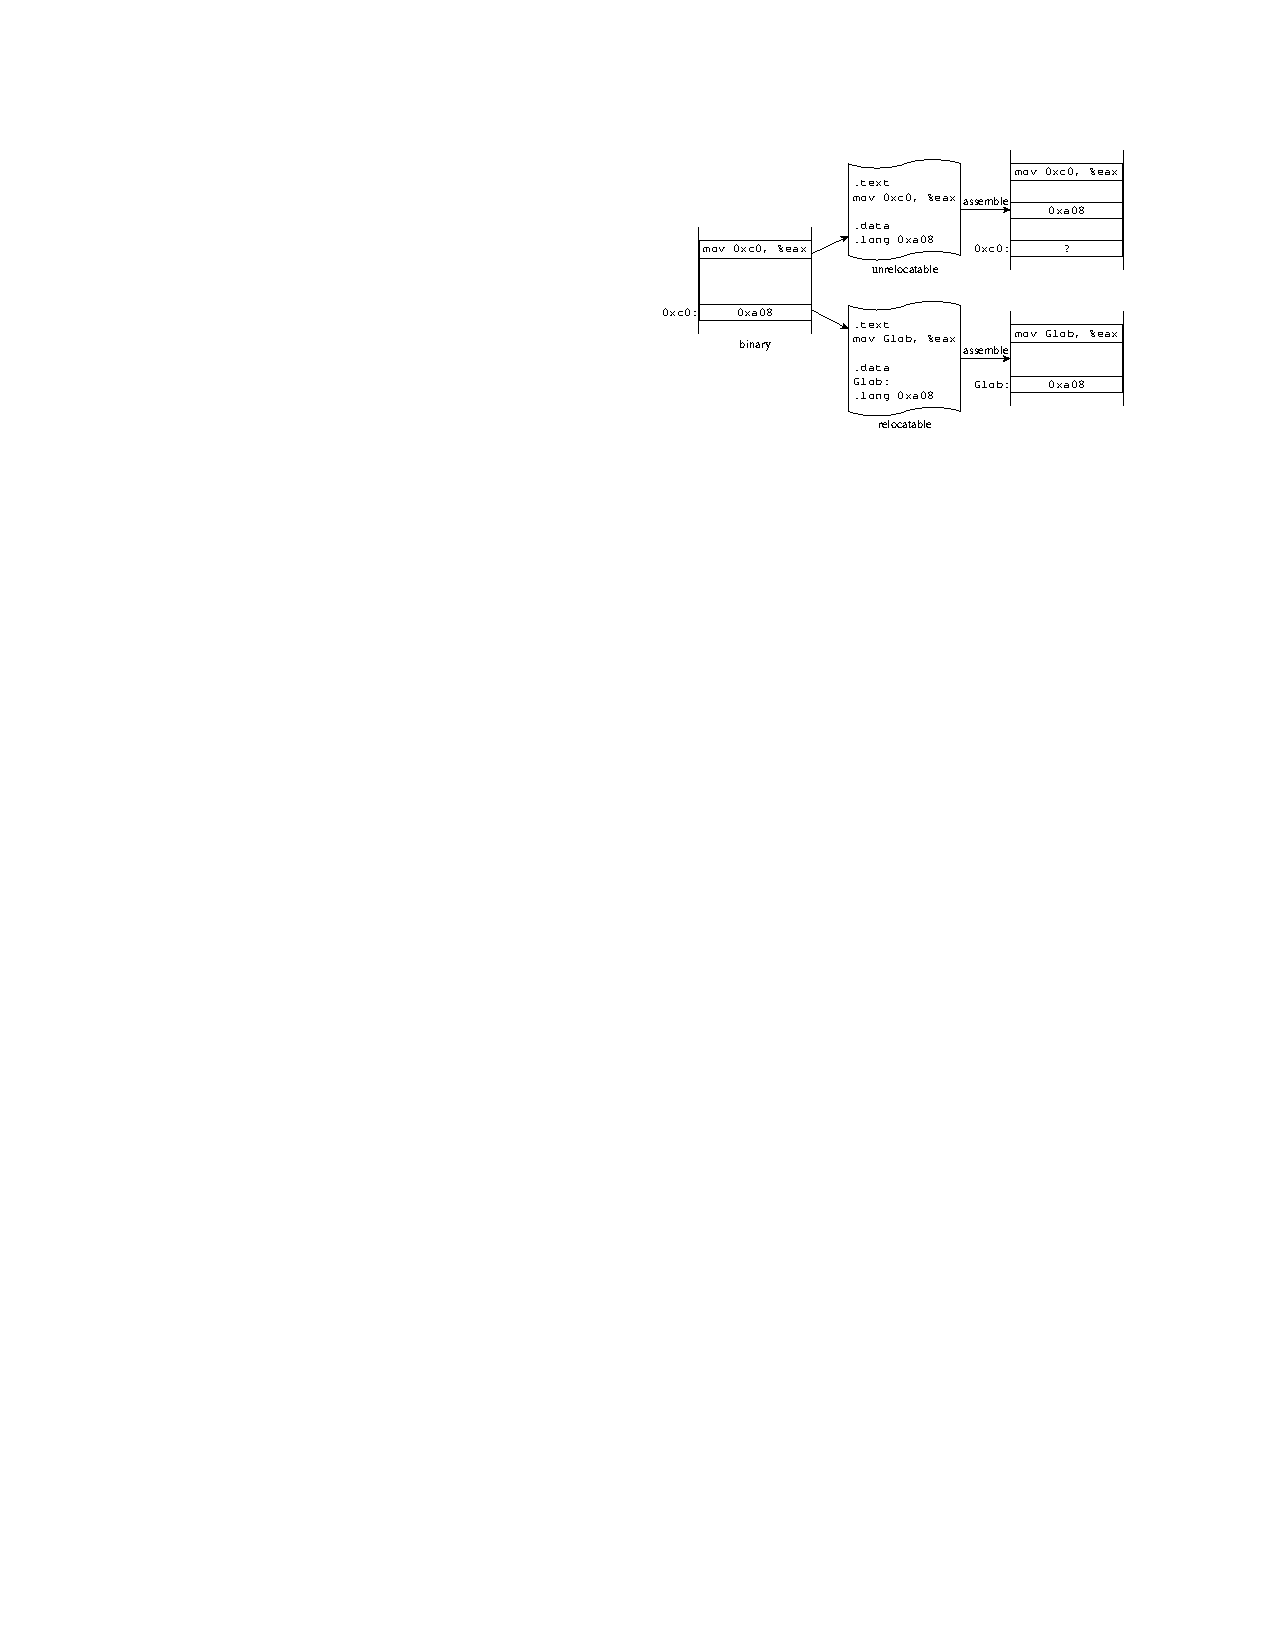
\includegraphics[width=0.8\textwidth]{fig/relocatable.pdf}
  \caption{Relocatable and unrelocatable assembly code~\cite{wang2015reassembleable}.}
  \label{fig:relocatable}
\end{figure}

\section{Variables Recovery} \label{sec:challenges-variable}
TODO

\section{Types Recovery} \label{sec:challenges-types}
TODO

\section{Control-Flow Recovery} \label{sec:challenges-control-flow}
TODO

\noindent\rule{8cm}{0.4pt}

\newpage
